\documentclass{beamer}
\usepackage[latin1]{inputenc}
\usepackage[3D]{movie15}
%\usetheme{Antibes}
\usetheme{Warsaw}
%\usetheme{Marburg}
%\usetheme[secheader]{Boadilla}
%\usetheme{default}
%\usetheme{Dresden}
%\usetheme{Madrid}
%\usetheme{Singapore}
\usecolortheme{seahorse}
%\usecolortheme{crane}
%\usecolortheme{albatross}
%\usecolortheme{whale}
%\usecolortheme{beaver}
%\usecolortheme{dolphin}
%\usecolortheme{seagull}

\usefonttheme{structuresmallcapsserif}
%\usefonttheme{structurebold}

\title[Machine Learning for Anatomical Neuroimaging]{Machine Learning for Anatomical Neuroimaging}
\author{John Ashburner}
\institute[j.ashburner@ucl.ac.uk]{Wellcome Trust Centre for Neuroimaging,\\
UCL Institute of Neurology,\\
12 Queen Square,\\
London WC1N 3BG,\\
UK.}
\date{}
\begin{document}

\begin{frame}
\titlepage
\end{frame}

\section{Introduction}
    \subsection{Why apply pattern recognition to structural MRI?} \begin{frame}
%\frametitle{There is more than just classification}
%\frametitle{To explain or to predict?}
\begin{center}
{\huge ``\emph{The only relevant test of the validity of a hypothesis is comparison of prediction with experience}.''\par}
\vspace{1cm}
Milton Friedman
\end{center}
\end{frame}

%\begin{frame}
%\frametitle{To explain or to predict?}

%\begin{quote}
%``The predictive point of view is a prototypical point of view to explain the basic activity of statistical analysis.''
%\par \rightline{\tiny{\rm --- Akaike}}
%\end{quote}

%\begin{quote}
%``The only useful function of a statistician is to make predictions.''
%\par \rightline{\tiny{\rm --- Deming}}
%\end{quote}

%\begin{quote}
%``The prediction of observables or potential observables is of much greater relevance than the estimate of what are often artificial constructs-parameters''
%\par\rightline{\tiny{\rm --- Geisser}}
%\end{quote}
%\vspace{.25cm}
%\begin{center}
%\begin{tiny}
%Galit Shmueli. ``To Explain or to Predict?''. Statistical Science 25(3):289--310 (2010).
%\end{tiny}
%\end{center}
%\end{frame}

%\begin{frame}
%\frametitle{To explain or to predict?}
%\begin{quote}
%%I should like to say a little about Heisenberg's idea that you should not talk about what you can not measure, because many people talk about this idea without really understanding it.
%You can interpret this in the sense that the {\bf construct or inventions that you make must be of such a kind that the consequences that you compute are comparable with experiment} - that is, that you do not compute a consequence like a `moo must be three goos', when nobody knows what a moo or a goo is.
%%  Obviously that is no good.  But if the consequences can be compared to experiment, then that is all that is necessary.  It does not matter that moos and goos cannot appear in the guess.  You can have as much junk in the guess as you like, provided that the consequences can be compared with experiment.  This is not always fully appreciated...\\
%...\\
%....{\bf Science is only useful if it tells you about some experiment that has not been done; it is no good if it only tells you what just went on.}
%\par \rightline{\tiny{\rm --- Richard Feynman; The Character of Physical Law}}
%\end{quote}
%\end{frame}


%\begin{frame}
%\frametitle{Choosing models/hypotheses/theories}
%\begin{columns}[c]
%\column{.3\textwidth}
%\includegraphics[width=\textwidth]{mackay}
%\vspace{.5cm}
%{\small
%MacKay, DJC. ``Bayesian interpolation.'' Neural computation 4, no. 3 (1992): 415-447.\par}
%\column{.7\textwidth}
%\includegraphics[width=\textwidth]{mackay1992}
%\end{columns}
%\end{frame}

\begin{frame}
\frametitle{Evidence-based Science}
...also just known as ``science''.
\vspace{0.5cm}
\begin{itemize}
\item{Researchers claim to find differences between groups.  Do those findings actually discriminate?}
\item{How can we most accurately diagnose a disorder from image data?}
\item{Pharma wants biomarkers.  How do we most effectively identify them?}
\item{There are lots of potential imaging biomarkers.  Which are most (cost) effective?}
\end{itemize}

Pattern recognition provides a framework to compare data (or preprocessing strategy) to determine the most accurate approach.
\end{frame}

\begin{frame}
\frametitle{Inter-subject Variability}
Why focus on anatomy?
\begin{itemize}
\item{Many medical applications involve understanding differences among individuals/populations.}
\item{In image data, most of the differences we can see are anatomical in nature.}
\item{Understanding growth and development requires us to look at growth and development (anatomy).}
\end{itemize}
\end{frame}

%\begin{frame}
%\frametitle{Cause and Effect}
%\begin{itemize}
%\item Anatomical data are generally purely observational (ie there's no intervention).
%\item Usually not possible to determine causality from such data.
%\item Causality is useful because it tells us something about outcomes from interventions.
%\item Usually in science, we predict dependent data (effects) from independent data (causes).
%\end{itemize}
%\end{frame}

\begin{frame}
\frametitle{Bayesian approaches may be better for clinical applications}
\begin{itemize}
\item Deals with different priors.
\begin{itemize}
\item Consider a method with 90\% sensitivity and specificity.
\item Consider using this to screen for a disease afflicting 1\% of the population.
\item On average, out of 100 people there would be 10 wrongly assigned to the disease group.
\item A positive diagnosis suggests only about a 10\% chance of having the disease.
{\small
\begin{eqnarray*}
P(\text{Disease} | \text{Pred+}) & = \frac{P(\text{Pred+} | \text{Disease}) P(\text{Disease})}{P(\text{Pred+} | \text{Disease}) P(\text{Disease}) + P(\text{Pred+} | \text{Healthy}) P(\text{Healthy})}\cr
% & = \frac{\text{Sensitivity} \times P(\text{Disease})}{\text{Sensitivity} \times P(\text{Disease}) + (1-Specificity) \times P(\text{Healthy})}
\end{eqnarray*}
\par
}
\end{itemize}
\item Better decision-making by accounting for utility functions.
\item Confidence may differ from subject to subject.
\end{itemize}
\end{frame}

%\begin{frame}
%\frametitle{Decision-making under uncertainty}
%\begin{itemize}
%\item Clinical decision-making is like gambling.
%\item Optimal way to gamble is Bayesian.
%\item ``Dutch Book Theorem''.
%\end{itemize}
%\end{frame}


    \subsection{Common ways to represent anatomical features}     \begin{frame}
\frametitle{Feature engineering}
\emph{First-timers are often surprised by how {\bf little time in a machine learning project is spent actually doing machine learning}.
But it makes sense if you consider how time-consuming it is to gather data, integrate it, clean it and pre-process it, and how much {\bf trial and error can go into feature design}.
Also, machine learning is not a one-shot process of building a data set and running a learner, but rather an iterative process of running the learner, analyzing the results, modifying the data and/or the learner, and repeating.
Learning is often the quickest part of this, but that's because we've already mastered it pretty well!
{\bf Feature engineering is more difficult because it's domain-specific, while learners can be largely general-purpose.}
However, there is no sharp frontier between the two, and this is another reason {\bf the most useful learners are those that facilitate incorporating knowledge}.
}

\vspace{1cm}
\begin{tiny}
Domingos, Pedro. ``A few useful things to know about machine learning.'' Communications of the ACM 55, no. 10 (2012): 78-87.\par
\end{tiny}
\end{frame}

\begin{frame}
\frametitle{Region volumes}
\begin{columns}[c]
\column{0.33\textwidth}
Label propagation or other methods can be used to subdivide brain into regions.\par

\column{0.67\textwidth}
\includegraphics[width=\textwidth]{brain-regions}
\end{columns}
\end{frame}

\begin{frame}
\frametitle{Pixel values}
\begin{columns}[c]
\column{0.33\textwidth}
Raw pixel data could be another option.\par
Data needs to be ``spatially normalised'' (and possibly skull-stripped).\par
Results may not generalise well to data from other scanners.\par
\column{0.67\textwidth}
\includegraphics[width=\textwidth]{brain-raw}
\end{columns}
\end{frame}

\begin{frame}
\frametitle{Tissue maps}
\begin{columns}[c]
\column{0.33\textwidth}
Grey matter maps can work fairly well.\par
Data needs to be ``spatially normalised''.\par
Many neurological problems show up as grey matter atrophy.\par
\column{0.67\textwidth}
\includegraphics[width=\textwidth]{brain-GM}
\end{columns}
\end{frame}

\begin{frame}
\frametitle{Other features}
\begin{columns}[c]
\column{0.33\textwidth}
Other features include:
\begin{itemize}
\item Cortical thickness.
\item Shape features.
\item Principal / Independent component weights.
\item Lesion maps.
\item etc
\end{itemize}
\column{0.67\textwidth}
\includegraphics[width=\textwidth]{brain-raw}
\end{columns}
\end{frame}


    \subsection{No Free Lunch and prior knowledge}                \begin{frame}
\frametitle{No Free Ducklings}
{\bf No Free Lunch theorem} says that learning is impossible without prior knowledge (\url{http://en.wikipedia.org/wiki/No\_free\_lunch\_in\_search\_and\_optimization}).

{\bf Ugly Duckling theorem} says that things are all equivalently similar to each other without prior knowledge (\url{http://en.wikipedia.org/wiki/Ugly\_duckling\_theorem}).

\vspace{1cm}
What prior knowledge do we have about the variability among people that can be measured using MRI?

How do we use this knowledge?
\end{frame}

\begin{frame}
\frametitle{Different ways of measuring distances}
\begin{columns}[c]
\column{.3\textwidth}
\includegraphics[width=\textwidth]{mumford}
\column{.7\textwidth}
\includegraphics[width=\textwidth]{mumford_fig}
\end{columns}
\end{frame}

%\begin{frame}
%\frametitle{Different ways of measuring distances}
%\begin{columns}[c]
%\column{.2\textwidth}
%\begin{center}
%Two simulated images\par
%\includegraphics[width=\textwidth]{figure2Di}
%\end{center}
%\column{.8\textwidth}
%\includegraphics[width=\textwidth]{figure2Dii}
%\end{columns}
%\end{frame}

\begin{frame}
\frametitle{Weighting the data}
\begin{Huge}
\begin{align*}
{\bf K} = {\bf X}{\bf W}{\bf X}^T
\end{align*}
\end{Huge}
\end{frame}

\begin{frame}
\frametitle{Prior knowledge about brain regions involved}
\begin{itemize}
\item The best way would be to augment the training data with data from previous studies.
\item Lack of data-sharing means this is generally not possible,\\
      so we need to extract information from publications.
\item The neuroimaging literature is mostly blobs.
\item These give pointers about how best to weight the data\\
      (${\bf W} = diag({\bf w}), w_i \in \mathbb{R}^+$).
\end{itemize}
\end{frame}

\begin{frame}
\frametitle{Weighting suspected regions more heavily}
\begin{center}
\includegraphics[width=.45\textwidth]{prior_knowledge_AD_NC}
\includegraphics[width=.45\textwidth]{prior_knowledge_MCI_NC}\par
\begin{tiny}
Chu et al. ``Does feature selection improve classification accuracy? Impact of sample size and feature selection on classification using anatomical magnetic resonance images''.  NeuroImage 60:59--70 (2012).\par
\end{tiny}
\end{center}
\end{frame}


    \subsection{Dimensionality reduction}                         
\begin{frame}
\frametitle{Curse of dimensionality}
\begin{center}
{\Huge Large $p$, small $n$.\par}
\end{center}
\end{frame}

\begin{frame}
\frametitle{Nearest-neighbour classification}
\begin{columns}[c]
\column{0.7\textwidth}
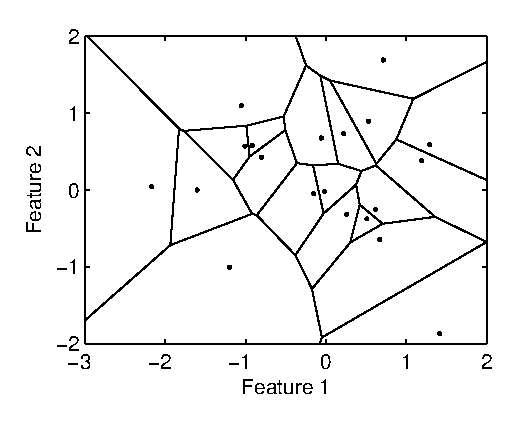
\includegraphics[width=\textwidth]{voronoi}
\column{0.3\textwidth}
\begin{itemize}
\item Not nice smooth separations.
\item Lots of sharp corners.
\item May be improved with \emph{K-nearest neighbours}.
\end{itemize}
\end{columns}
\end{frame}

\begin{frame}
\frametitle{Rule-based approaches}
\begin{columns}[c]
\column{0.7\textwidth}
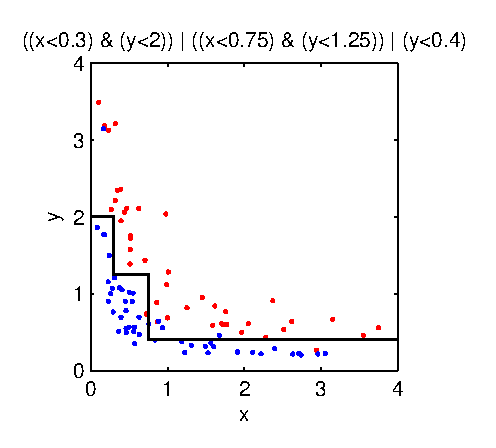
\includegraphics[width=\textwidth]{rule_based}
\column{0.3\textwidth}
\begin{itemize}
\item Not nice smooth separations.
\item Lots of sharp corners.
\end{itemize}
\end{columns}
\end{frame}


\begin{frame}
\frametitle{Corners matter in high-dimensions}
\begin{columns}[c]
\column{0.4\textwidth}
\includegraphics[width=\textwidth]{circle}
\column{0.6\textwidth}
\includegraphics[width=\textwidth]{sphere}
\end{columns}
\end{frame}

\begin{frame}
\frametitle{Corners matter in high-dimensions}
\begin{columns}[c]
\column{0.2\textwidth}
\includegraphics[width=.8\textwidth]{circle}

\includegraphics[width=\textwidth]{sphere}
\column{0.8\textwidth}
\includegraphics[width=\textwidth]{corners}
\end{columns}
\end{frame}


\begin{frame}
\frametitle{Dimensionality $\ne$ number of voxels}
\begin{itemize}
\item Lots of effort on data-driven feature selection methods.
\begin{itemize}
\item Involves estimating weighting matrix such that\\
      ${\bf W} = diag({\bf w}), w_i \in \{0,1\}$.
\item Lots of parameters needed to achieve this.
\end{itemize}
\item Many papers claim excellent results.
\item Little evidence to suggest that most voxel-based feature selection methods help.
\begin{itemize}
\item Little or no increase in predictive accuracy.
\item Commonly perceived as being more ``interpretable''.
\end{itemize}
%\item Prior knowledge derived from independent data is the most reliable way to improve accuracy.
%\begin{itemize}
%\item e.g. search the literature for clues about which regions to weight more heavily.
%\end{itemize}
\end{itemize}
\end{frame}

\begin{frame}
%\frametitle{Credentials}
\begin{center}
\includegraphics[height=0.7\textwidth]{pbaic2007}
\end{center}
\end{frame}

\begin{frame}
%\frametitle{Credentials}
\begin{center}
\includegraphics[height=0.7\textwidth]{pbaic2007_2}
\end{center}
\end{frame}


%\begin{frame}
%\frametitle{Data-driven feature selection}
%\begin{itemize}
%\item Lots of effort on data-driven feature selection methods.
%\item Many papers claim excellent results.
%\item Not much evidence that it really improves accuracy.
%\end{itemize}
%\end{frame}

\begin{frame}
\frametitle{Data-driven feature selection}
%The main objectives of the feature selection step are to keep only informative features and to reduce the dimensionality of the feature space.
\begin{quote}
``In our evaluation, two methods included a feature selection step: Voxel-STAND and Voxel-COMPARE.
Overall, these methods did not perform substantially better than simpler ones... ...
%In particular, their results might be more sensitive to the training set.
%Indeed, feature selection can be regarded as a learning step.
%In such a case, the feature selection step increases the class of all possible classification functions, which could lead to overfitting the data.
A more robust way to decrease the dimensionality of the features way would be to use more prior knowledge of the disease.''

%Besides features selection can be time consuming as it adds new hyperparameters and thus makes the grid search less tractable.
%Compared to Voxel-Direct and Voxel-Atlas, Voxel-STAND and Voxel-COMPARE are time consuming (up to weeks), mostly because of the number of hyperparameters to be tuned.

%Nevertheless, feature selection proved useful in two specific cases.
%First, these methods proved less sensitive when increasing the dimensionality of the feature space by adding WM and CSF maps.
%They also tended to be more accurate for the MCIc vs MCInc experiment, where only a few brain regions are informative.
\end{quote}

\begin{center}
\begin{tiny}
Cuingnet et al. ``Automatic classification of patients with Alzheimer's disease from structural MRI: A comparison of ten methods using the ADNI database''.  NeuroImage 56(2):766--781 (2011).\par
\end{tiny}
\end{center}
\end{frame}

\begin{frame}
\frametitle{Data-driven feature selection}
\begin{center}
\includegraphics[height=0.55\textwidth]{data_driven_feature_selection.png}\par
\begin{tiny}
Chu et al. ``Does feature selection improve classification accuracy? Impact of sample size and feature selection on classification using anatomical magnetic resonance images''.  NeuroImage 60:59--70 (2012).\par
\end{tiny}
\end{center}
\end{frame}

\begin{frame}
\frametitle{One mode of geometric variability}
\begin{columns}[c]
\column{0.5\textwidth}
Simulated images\par
\includegraphics[height=0.9\textwidth]{circles}
\column{0.5\textwidth}
Principal components\par
\includegraphics[height=0.9\textwidth]{circles_pca}
\end{columns}
A suitable model would reduce these data to a single dimension.
\end{frame}


\begin{frame}
\frametitle{Two modes of geometric variability}
\begin{columns}[c]
\column{0.5\textwidth}
Simulated images\par
\includegraphics[height=0.9\textwidth]{things}
\column{0.5\textwidth}
Principal components\par
\includegraphics[height=0.9\textwidth]{things_pca}
\end{columns}
A suitable model would reduce these data to two dimensions.
\end{frame}



\section{Geometric Morphometrics}
    \subsection{Early univariate morphometry}                     \include{EarlyUnivariateMorphometry}
    \subsection{Early multivariate morphometry}                   \include{EarlyMultivariateMorphometry}
    \subsection{The morphometrics ``revolution'' (landmarks)}     \include{TheMorphometricsRevolution}
    \subsection{Allometric relations}                             \include{AllometricRelations}
    \subsection{Automated shape estimation}                       \begin{frame}
\frametitle{Non-Euclidean geometry}
\begin{columns}[c]
\column{0.5\textwidth}
\begin{itemize}
\item Distances are not always measured along a straight line.
\item ``\emph{Shapes are the ultimate non-linear sort of thing}''
\end{itemize}
\column{0.5\textwidth}
\includegraphics[width=\textwidth]{Globe}
\end{columns}
\end{frame}

\begin{frame}
\frametitle{Linear approximations to nonlinear problems}
%\begin{columns}[c]
%\column{0.2\textwidth}
%Dealing with non-Euclidean geometry.
%Linear approximation around the average.
%\begin{center}
%\column{0.8\textwidth}
\begin{center}
\includegraphics[width=1.2\textwidth]{spheres}
\end{center}
%\end{columns}
\end{frame}

%\begin{frame}
%\frametitle{D'Arcy Thompson's Generative Model}
%\begin{quote}
%``...diverse and dissimilar fishes can be referred as a whole to identical functions of very different co-ordinate systems...''
%\end{quote}
%\begin{center}
%\includegraphics[height=0.4\textheight]{OGAF}
%\includegraphics[height=0.4\textheight]{fish}
%\end{center}
%We can compute relative shapes using image registration.
%\end{frame}



\section{Similarity between brains}
    \subsection{Distances between anatomies}                      %\begin{frame}
%\frametitle{Nonlinearity of Shapes}
%\begin{columns}[c]
%\column{0.7\textwidth}
%According to David Mumford (Fields Medal, 1974):
%\begin{quote}
%``Shapes are the ultimate non-linear sort of thing''
%\end{quote}
%
%Relative shapes can not be added and subtracted (ie, they are nonlinear).
%Instead, deformations should combined by composing them together.
%
%Deformations that are smooth and invertible are known as \emph{diffeomorphisms}, and form a mathematical \emph{group}.
%
%\column{0.3\textwidth}
%\includegraphics[height=.8\textheight]{2Dpics}
%\end{columns}
%\end{frame}


    \subsection{Non-linear distances (manifolds)}                 \begin{frame}
\frametitle{Non-Euclidean geometry}
\begin{columns}[c]
\column{0.8\textwidth}
\begin{itemize}
\item Distances are not always measured along a straight line.\par
\item Sometimes we want distances measured on a manifold.\par
\item Shortest path on a manifold is along a \emph{geodesic}.
\end{itemize}
\column{0.2\textwidth}
\includegraphics[width=\textwidth]{Globe}
\end{columns}

\vspace{0.25cm}
Linear trajectory\par
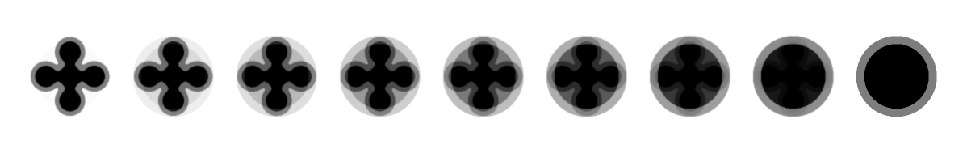
\includegraphics[width=\textwidth]{series1}\par
Nonlinear trajectory\par
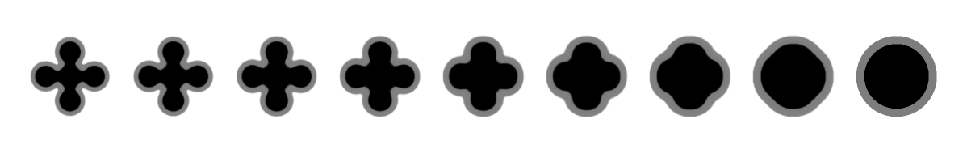
\includegraphics[width=\textwidth]{series2}\par
\end{frame}

%\begin{frame}
%\frametitle{Metric distances}
%Fly in a straight line, but the path is curved.\par
%\begin{center}
%\includegraphics[width=.9\textwidth]{NewYork-London}
%\end{center}
%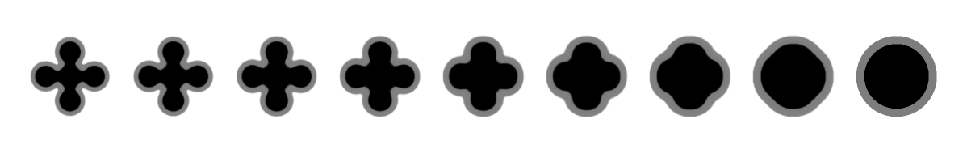
\includegraphics[width=\textwidth]{series2}\par
%\end{frame}


\begin{frame}
\frametitle{Metric distances}
Distances should satisfy the properties of a \emph{metric}:
\begin{enumerate}
\item $d({\bf x}, {\bf y}) \ge 0$ (non-negativity)
\item $d({\bf x}, {\bf y}) = 0$ if and only if ${\bf x} = {\bf y}$ (identity of indiscernibles)
\item $d({\bf x}, {\bf y}) = d({\bf y}, {\bf x})$ (symmetry)
\item $d({\bf x}, {\bf z}) \le d({\bf x}, {\bf y}) + d({\bf y}, {\bf z})$ (triangle inequality).
\end{enumerate}

Satisfying (3) requires inverse-consistent image registration.

Satisfying (4) requires a specific class of image registration models.

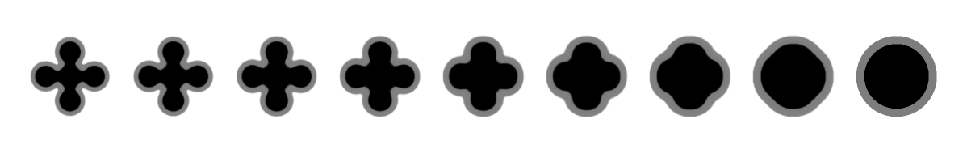
\includegraphics[width=\textwidth]{series2}\par
\end{frame}

\begin{frame}
\frametitle{Computing a metric distance}
\includegraphics[width=\textwidth]{trajectory0}\par
\begin{columns}[c]
\column{0.8\textwidth}
Decompose a curved path into a series of short line segments, and add the lengths of the segments together.\par
\column{0.2\textwidth}
\includegraphics[width=\textwidth]{Globe}
\end{columns}
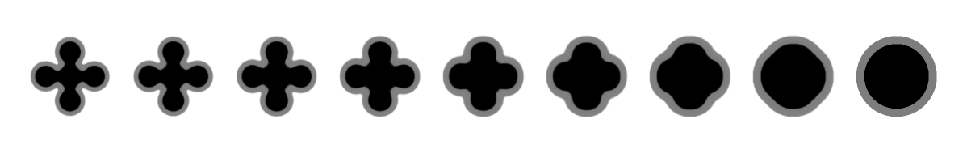
\includegraphics[width=\textwidth]{series2}
\end{frame}


%%%%%%%%%%%%%%%%%%%%%%%%%%%%%%%%%%%%%%%%%%%%%%%%%%%%%%%%%%%%%%%
\begin{frame}
\frametitle{Computing large deformations}
\includegraphics[width=\textwidth]{trajectory0}\par
We can consider a large deformation as the composition of a series of small deformations:
\begin{eqnarray*}
{\boldsymbol\varphi}_{1} = \left(\mathrm{id} + \tfrac{{\bf v}_{t_{N-1}}}{N}\right) \circ  \left(\mathrm{id} + \tfrac{{\bf v}_{t_{N-2}}}{N}\right) \circ ... \circ \left(\mathrm{id} + \tfrac{{\bf v}_{t_1}}{N}\right) \circ \left(\mathrm{id} + \tfrac{{\bf v}_0}{N}\right)
\end{eqnarray*}

The inverse of the deformation can be computed from:
\begin{eqnarray*}
{\boldsymbol\vartheta}_{1} = \left(\mathrm{id} - \tfrac{{\bf v}_0}{N}\right) \circ  \left(\mathrm{id} - \tfrac{{\bf v}_{t_1}}{N}\right) \circ ... \circ \left(\mathrm{id} - \tfrac{{\bf v}_{t_{N-2}}}{N}\right) \circ \left(\mathrm{id} - \tfrac{{\bf v}_{t_{N-1}}}{N}\right)
\end{eqnarray*}

\end{frame}

%%%%%%%%%%%%%%%%%%%%%%%%%%%%%%%%%%%%%%%%%%%%%%%%%%%%%%%%%%%%%%%

\begin{frame}
\frametitle{Metric distances from large deformations}
By modelling trajectories as piecewise linear, distances can be computed by adding the distances from the small deformations:
\begin{eqnarray*}
d = \frac{1}{N}\sum_{n=0}^{N-1} || {\bf L} {\bf v}_{t_n} ||
\end{eqnarray*}
%\includegraphics[width=\textwidth]{trajectory0}

If $N$ approaches infinity (and we use small deformations of $\mathrm{id} + \frac{1}{N}{\bf v}_t$), the evolution of a deformation may be conceptualised as integrating the following equation:
\begin{eqnarray*}
\frac{d {\boldsymbol\varphi}}{d t} = {\bf v}_t ({\boldsymbol\varphi})
\end{eqnarray*}

Geodesic distances (from zero) are then measured by:
\begin{eqnarray*}
d = \int_{t=0}^1  || {\bf L} {\bf v}_t || dt
\end{eqnarray*}
\end{frame}

\begin{frame}
\frametitle{Metric distances from large deformations}
\includegraphics[width=\textwidth]{hippocampi}\par
\begin{tiny}
Miller et al. ``Collaborative computational anatomy: an MRI morphometry study of the human brain via diffeomorphic metric mapping.'' Human Brain Mapping 30(7):2132--2141 (2009).\par
\end{tiny}
\end{frame}

\begin{frame}
\frametitle{Metric distances from large deformations}
\includegraphics[width=.8\textwidth]{metric_distances}\par
\begin{tiny}
Miller et al. ``Collaborative computational anatomy: an MRI morphometry study of the human brain via diffeomorphic metric mapping.'' Human Brain Mapping 30(7):2132--2141 (2009).\par
\end{tiny}
\end{frame}


    \subsection{Image registration for measuring distances}       \begin{frame}
\frametitle{Image Registration}
\begin{columns}[c]
\column{0.7\textwidth}
\begin{itemize}
\item Image registration measures distances between images.
\item Often involves minimising the sum of two terms:
\begin{itemize}
\item Distance between the image intensities.
\item Distance of the deformation from the identity.
\end{itemize}
\item The sum of these terms gives the distance.
\end{itemize}
\column{0.3\textwidth}
\includegraphics[width=\textwidth]{shoot2d}
\end{columns}
\end{frame}

%%%%%%%%%%%%%%%%%%%%%%%%%%%%%%%%%%%%%%%%%%%%%%%%%%%%%%%%%%%%%%%
\begin{frame}
\frametitle{LDDMM}
\emph{Large Deformation Diffeomorphic Metric Mapping} is an image registration algorithm that minimises the following:
\begin{eqnarray*}
\mathcal{E}  =   \frac{1}{2} \int_{t=0}^1  || {\bf L} {\bf v}_t ||^2 dt +
                 \frac{1}{2\sigma^2} || f - \mu\left({\boldsymbol\varphi}_1^{-1}\right)||^2\\
\text{  where } {\boldsymbol\varphi}_0 = \mathrm{Id} \text{, } \frac{d{\boldsymbol\varphi}}{dt} = {\bf v}_t\left({\boldsymbol\varphi}_t\right)
\end{eqnarray*}

The first term minimises the squared distance measure of the deformations, whereas the second term simply minimises the difference between the warped template and the individual scan.

The objective is to estimate a series of velocity fields (${\bf v}_t$).\par
%\includegraphics[width=\textwidth]{trajectory}
%These may be conceptualised as
%\begin{eqnarray*}
%\frac{d {\boldsymbol\varphi}}{d t} = {\bf v}_t ({\boldsymbol\varphi})
%\end{eqnarray*}
\vspace{.25cm}
\begin{tiny}
Beg, MF, Miller, MI, Trouv{\'e}, A \& Younes, L. \emph{Computing large deformation metric mappings via geodesic flows of diffeomorphisms}. International Journal of Computer Vision 61(2):139--157 (2005).

\end{tiny}

\end{frame}

%%%%%%%%%%%%%%%%%%%%%%%%%%%%%%%%%%%%%%%%%%%%%%%%%%%%%%%%%%%%%%%

%\begin{frame}
%\frametitle{Different ways of measuring distances}
%\begin{columns}[c]
%\column{.2\textwidth}
%\begin{center}
%Two simulated images\par
%\includegraphics[width=\textwidth]{figure2Di}
%\end{center}
%\column{.8\textwidth}
%\includegraphics[width=\textwidth]{figure2Dii}
%\end{columns}
%\end{frame}



%\begin{frame}
%\frametitle{Change of Variables}
%When we warp images, we should usually account for expansion/contraction via a change of variables.
%\begin{eqnarray*}
%\int_{{\bf x} \in \varphi(\Omega)} f({\bf x}) d{\bf x} = \int_{{\bf x} \in \Omega} f(\varphi({\bf x})) \det |({\bf D}\varphi)({\bf x})| d{\bf x}
%\end{eqnarray*}
%where $({\bf D}\varphi)({\bf x})$ means the Jacobian of $\varphi$ at ${\bf x}$.
%\end{frame}

%%%%%%%%%%%%%%%%%%%%%%%%%%%%%%%%%%%%%%%%%%%%%%%%%%%%%%%%%%%%%%%

%\begin{frame}
%\frametitle{LDDMM}
%Estimating a series of velocity fields looks like it involves estimating a lot of parameters, but this is not actually the case.
%\includegraphics[width=\textwidth]{trajectory}

%The matching term of the objective function is:
%\begin{eqnarray*}
%\frac{1}{2\sigma^2} \int_{x\in\Omega} ( f \circ {\bf x} - \mu \circ {\boldsymbol\varphi}_{1}^{-1} \circ {\bf x})^2 d{\bf x}
%\end{eqnarray*}

%This may be re-written (including a change of variables) as:
%\begin{eqnarray*}
%\frac{1}{2\sigma^2} \int_{x\in\Omega} \det |{\bf D}( {\boldsymbol\varphi}_{1} \circ {\boldsymbol\varphi}_{t}^{-1}) \circ {\bf x} | ( f \circ {\boldsymbol\varphi}_1 \circ {\boldsymbol\varphi}_{t}^{-1} \circ {\bf x} - \mu \circ {\boldsymbol\varphi}_{t}^{-1} \circ {\bf x})^2 d{\bf x}
%\end{eqnarray*}
%This allows the derivatives of the matching term to be computed at any time point.
%\end{frame}


    \subsection{Tangent space representations}                    \begin{frame}
\frametitle{Linear approximations to nonlinear problems}
%\begin{columns}[c]
%\column{0.2\textwidth}
%Dealing with non-Euclidean geometry.
%Linear approximation around the average.
%\begin{center}
%\column{0.8\textwidth}
\begin{center}
\includegraphics[width=\textwidth]{spheres}
\end{center}
%\end{columns}
\end{frame}

\begin{frame}
\frametitle{Exponential map}
\begin{columns}[c]
\column{0.6\textwidth}
\includegraphics[width=\textwidth]{900px-Azimuthal_Equidistant_N90}
\column{0.4\textwidth}
\begin{center}
\includegraphics[width=\textwidth]{spheres}
\end{center}
\begin{tiny}
``Azimuthal Equidistant N90'' by RokerHRO - Own work. Licensed under CC BY-SA 3.0 via Wikimedia Commons - \url{http://commons.wikimedia.org/wiki/File:Azimuthal\_Equidistant\_N90.jpg}\par
\end{tiny}
\end{columns}
\end{frame}

\begin{frame}
\frametitle{LDDMM via ``geodesic shooting''}
\begin{columns}[c]
\column{0.65\textwidth}
In practice, we just need to estimate an initial velocity (${\bf v}_0$), from which we compute the initial momentum by ${\bf u}_0 = {\bf L}^{\dagger}{\bf L}{\bf v}_0$.

We set the deformation at time 0 to an identity transform (${\boldsymbol\varphi}_0 = Id$), and then evolve the following dynamical system for unit time:
\begin{eqnarray*}
{\bf u}_{t} = & \det |{\bf D}{\boldsymbol\varphi}_{t}^{-1}| ({\bf D}{\boldsymbol\varphi}_{t}^{-1})^T ({\bf u}_{0} \circ {\boldsymbol\varphi}_{t}^{-1})\cr
{\bf v}_{t} = & \left({\bf L}^{\dagger}{\bf L}\right)^{-1} {\bf u}_t\cr
\frac{d {\boldsymbol\varphi}}{d t} = & {\bf v}_t ({\boldsymbol\varphi}_t)
\end{eqnarray*}
\column{0.35\textwidth}
\begin{center}
\includegraphics[width=1\textwidth]{evolution1}
\end{center}
\end{columns}
\vspace{.25cm}
\begin{tiny}
Younes, L, Arrate, F \& Miller, MI. \emph{Evolutions equations in computational anatomy}. Neuroimage 45(1S1):40--50 (2009).\par
\end{tiny}
\end{frame}


\begin{frame}
\frametitle{LDDMM via ``geodesic shooting''}
\begin{columns}[c]
\column{0.65\textwidth}
The final deformation (${\boldsymbol\varphi}_1$) is a type of exponential of the initial velocity (${\bf v}_0$).
\vspace{0.25cm}
\begin{tiny}
Exponential map (Riemannian geometry). (2015, January 13). In Wikipedia, The Free Encyclopedia. Retrieved 18:04, March 31, 2015, from \url{http://en.wikipedia.org/w/index.php?title=Exponential\_map\_(Riemannian\_geometry)\&oldid=642372186}\par
\end{tiny}
\column{0.35\textwidth}
\begin{center}
\includegraphics[width=1\textwidth]{evolution1}
\end{center}
\end{columns}

\vspace{.25cm}
\begin{tiny}
Younes, L, Arrate, F \& Miller, MI. \emph{Evolutions equations in computational anatomy}. Neuroimage 45(1S1):40--50 (2009).\par
\end{tiny}
\end{frame}


%%%%%%%%%%%%%%%%%%%%%%%%%%%%%%%%%%%%%%%%%%%%%%%%%%%%%%%%%%%%%%%

\begin{frame}
\frametitle{``Groupwise registration''}
Minimising distortions by centering around the mean.
\begin{center}
\includegraphics[width=.8\textwidth]{groupwise}
\end{center}
\end{frame}

\begin{frame}
\frametitle{``Groupwise registration''}
\begin{center}
\includegraphics[width=.7\textwidth]{aligned_ties}
\end{center}
\end{frame}

\begin{frame}
\frametitle{``Groupwise registration''}
\begin{columns}[c]
\column{0.3\textwidth}
Ignoring the many technical details, the procedure involves alternating between:
\begin{itemize}
\item Create the mean of aligned images.
\item Align all images to be slightly closer to the mean.
\end{itemize}
\column{0.7\textwidth}
\begin{center}
\includegraphics[height=.8\textheight]{groupwiseII}
\end{center}
\end{columns}
\end{frame}

\begin{frame}
\frametitle{Kernel matrix}
Construction of kernel matrix accounts for the regularisation used by the image registration:
\begin{Large}
\begin{align*}
k({\bf v},{\bf w}) & = \langle {\bf L}^{\dagger} {\bf L} {\bf v}, {\bf w} \rangle\cr
                   & = \langle {\bf L} {\bf v}, {\bf L} {\bf w} \rangle
\end{align*}
\end{Large}

\vspace{0.25cm}
\begin{tiny}
Wang, Lei, et al. ``Large deformation diffeomorphism and momentum based hippocampal shape discrimination in dementia of the Alzheimer type.'' Medical Imaging, IEEE Transactions on 26(4):462--470 (2007).\par
\end{tiny}
\end{frame}

%\begin{frame}
%\frametitle{D'Arcy Thompson's Generative Model}
%\begin{quote}
%``...diverse and dissimilar fishes can be referred as a whole to identical functions of very different co-ordinate systems...''
%\end{quote}
%\begin{center}
%\includegraphics[height=0.4\textheight]{OGAF}
%\includegraphics[height=0.4\textheight]{fish}
%\end{center}
%We can compute relative shapes using image registration.
%\end{frame}

% Top speed of an Airbus A380 is 1,020 km/h
% distance from NY:
% London 5576 km
% Los Angeles 3940 km

%\begin{frame}
%\frametitle{Kernel Matrices}
%Linear kernel matrices may computed from the raw features.
%\begin{eqnarray*}
%{\bf K} = {\bf X}{\bf X}^T
%\end{eqnarray*}
%A simple spatial feature selection may be considered as the following, where $\boldsymbol\Sigma_0$ is a diagonal matrix of ones and zeros:
%\begin{eqnarray*}
%{\bf K} = {\bf X}\boldsymbol\Sigma_0{\bf X}^T
%\end{eqnarray*}
%However, $\boldsymbol\Sigma_0$ may be more complicated, for example encoding spatial smoothing, high-pass filtering or any number of other things.
%\end{frame}

%\begin{frame}
%\frametitle{Inner Products}
%This gives us an alternative way of measuring distances between vectors in a linear way, where $\boldsymbol\Sigma_0$ is symmetric and positive definite.
%\begin{eqnarray*}
%d({\bf x}_1,{\bf x}_2) = \sqrt{({\bf x}_1 - {\bf x}_2)^T \boldsymbol\Sigma_0 ({\bf x}_1 - {\bf x}_2)}
%\end{eqnarray*}
%
%Usually, the operation $\boldsymbol\Sigma_0{\bf x}^T$ is performed as a convolution.  For example, when dealing with 2D data, we may convolve with the Laplacian operator.
%\begin{eqnarray*}
%{\nabla}^2 {\bf x} = {\bf x} \ast \begin{pmatrix} 0 & -1 & 0\cr -1 & 4 & -1\cr 0 & -1 & 0\end{pmatrix}
%\end{eqnarray*}
%
%Note that the actual form of $\boldsymbol\Sigma_0$ can vary, so we need to figure out what metric tensor is optimal.
%\end{frame}


    \subsection{Scalar momenta}                                   %\begin{frame}
%\frametitle{Euler-Lagrange Equations}
%At the solution, the derivatives of the objective function are zero, which means that the velocity at any time point is given by:
%\begin{eqnarray*}
%{\bf L}^{\dagger}{\bf L}{\bf v}_{t} = \frac{1}{\sigma^2} \det |{\bf D}( {\boldsymbol\varphi}_{1} \circ {\boldsymbol\varphi}_{t}^{-1}) | (\nabla (\mu \circ {\boldsymbol\varphi}_{t}^{-1})) (\mu \circ {\boldsymbol\varphi}_{t}^{-1} - f \circ {\boldsymbol\varphi}_1 \circ {\boldsymbol\varphi}_{t}^{-1}) 
%\end{eqnarray*}

%If we introduce something that we'll call initial momentum:
%\begin{eqnarray*}
%{\bf u}_{0} = {\bf L}^{\dagger}{\bf L} {\bf v}_0 = \frac{1}{\sigma^2} \det | {\bf D}{\boldsymbol\varphi}_{1} | (\nabla \mu) (\mu - f \circ {\boldsymbol\varphi}_1)
%\end{eqnarray*}
%we see that the velocity at any time point is determined by the initial momentum (or velocity), according to:
%\begin{eqnarray*}
%{\bf v}_{t} = \left({\bf L}^{\dagger}{\bf L}\right)^{-1} \left(\det |{\bf D}{\boldsymbol\varphi}_{t}^{-1}| ({\bf D}{\boldsymbol\varphi}_{t}^{-1})^T ({\bf u}_{0} \circ {\boldsymbol\varphi}_{t}^{-1}) \right)
%\end{eqnarray*}
%\end{frame}

\begin{frame}
\frametitle{Geodesic Shooting}
At the solution, gradients of the objective function should vanish:
\begin{align*}
{\bf L}^{\dagger}{\bf L} {\bf v}_{0} + \frac{1}{\sigma^2} \det | {\bf D}{\boldsymbol\varphi}_{1} | (f \circ {\boldsymbol\varphi}_1 - \mu)(\nabla \mu) = 0
\end{align*}

Re-expressiong this, we see that the initial velocity and momentum is given by:
\begin{align*}
{\bf L}^{\dagger}{\bf L} {\bf v}_{0} = {\bf u}_0 = {\frac{1}{\sigma^2} (\nabla \mu)} {\det | {\bf D}{\boldsymbol\varphi}_{1} | (\mu - f \circ {\boldsymbol\varphi}_1)}
\end{align*}
\end{frame}

%%%%%%%%%%%%%%%%%%%%%%%%%%%%%%%%%%%%%%%%%%%%%%%%%%%%%%%%%%%%%%%
\begin{frame}
\frametitle{``Scalar Momentum''}
\begin{eqnarray*}
{\bf u}_{0} = \color{blue}{\frac{1}{\sigma^2} (\nabla \mu)} \color{red}{\det | {\bf D}{\boldsymbol\varphi}_{1} | (\mu - f \circ {\boldsymbol\varphi}_1)}
\end{eqnarray*}
If a population of subjects are all aligned with the same template image, $\color{blue}{\frac{1}{\sigma^2} (\nabla \mu)}$ will be the same for all subjects.
Deviations from the template are encoded by the ``\emph{scalar momentum}'', $\color{red}{\det | {\bf D}{\boldsymbol\varphi}_{1} |(\mu - f \circ {\boldsymbol\varphi}_1)}$.
This is a scalar field, and in principle is all that is needed (along with the template) to reconstruct the original images.\par
\vspace{.25cm}
\begin{tiny}
Miller et al. ``Collaborative computational anatomy: an MRI morphometry study of the human brain via diffeomorphic metric mapping.'' Human Brain Mapping 30(7):2132--2141 (2009).\par
Singh, Fletcher, Preston, Ha, King, Marron, Wiener \& Joshi (2010). \emph{Multivariate Statistical Analysis of Deformation Momenta Relating Anatomical Shape to Neuropsychological Measures}. T. Jiang et al. (Eds.): MICCAI 2010, Part III, LNCS 6363, pp. 529--537, 2010.\par
\end{tiny}
\end{frame}

\begin{frame}
\frametitle{Evolution}
\begin{center}
\includegraphics[width=.9\textwidth]{evolution}
\end{center}
\end{frame}


%%%%%%%%%%%%%%%%%%%%%%%%%%%%%%%%%%%%%%%%%%%%%%%%%%%%%%%%%%%%%%%

\begin{frame}
\frametitle{Example Images}
Some example images.
\begin{center}
\includegraphics[width=0.9\textwidth]{original}
\end{center}
\end{frame}

%%%%%%%%%%%%%%%%%%%%%%%%%%%%%%%%%%%%%%%%%%%%%%%%%%%%%%%%%%%%%%%

\begin{frame}
\frametitle{Scalar Momentum}
Scalar momentum after aligning the examples to a common template.
\begin{center}
\includegraphics[width=0.9\textwidth]{alpha}
\end{center}
\end{frame}

%%%%%%%%%%%%%%%%%%%%%%%%%%%%%%%%%%%%%%%%%%%%%%%%%%%%%%%%%%%%%%%

\begin{frame}
\frametitle{Reconstructed Images}
Images reconstructed using just the template and scalar momentum.
\begin{center}
\includegraphics[width=0.9\textwidth]{reconstructed}
\end{center}
\end{frame}

%%%%%%%%%%%%%%%%%%%%%%%%%%%%%%%%%%%%%%%%%%%%%%%%%%%%%%%%%%%%%%%



    \subsection{Empirical examples}                               \begin{frame}
\frametitle{Real data}
\begin{columns}[c]
\column{0.5\textwidth}
Used 550 T1w brain MRI from IXI ({\bf I}nformation e{\bf X}traction from {\bf I}mages) dataset.\par
\url{http://www.brain-development.org/}\par
Data from three different hospitals in London:
\begin{itemize}
\item{Hammersmith Hospital using a Philips 3T system}
\item{Guy's Hospital using a Philips 1.5T system}
\item{Institute of Psychiatry using a GE 1.5T system}
\end{itemize}

\column{0.5\textwidth}
\includegraphics[width=0.9\textwidth]{orig_ixi}
\end{columns}
\end{frame}



\begin{frame}
\frametitle{Grey and White Matter}
\begin{columns}[c]
\column{0.26\textwidth}
Segmented into GM and WM.

Approximately aligned via rigid-body.
\column{0.75\textwidth}
\includegraphics[width=0.5\textwidth]{gm_ixi}
\includegraphics[width=0.5\textwidth]{wm_ixi}
\end{columns}

\begin{tiny}
Ashburner, J \& Friston, KJ. \emph{Unified segmentation}. NeuroImage 26(3):839--851 (2005).\par
\end{tiny}
\end{frame}



\begin{frame}
\frametitle{Diffeomorphic Alignment}
All GM and WM were diffeomorphically aligned to their common average-shaped template.
\begin{center}
\includegraphics[width=.8\textwidth]{template}
\end{center}

\begin{tiny}
Ashburner, J \& Friston, KJ. \emph{Diffeomorphic registration using geodesic shooting and Gauss-Newton optimisation}. NeuroImage 55(3):954--967 (2011).\par
Ashburner, J \& Friston, KJ. \emph{Computing average shaped tissue probability templates}. NeuroImage 45(2):333--341 (2009).\par
\end{tiny}
\end{frame}



\begin{frame}
\frametitle{Volumetric Features}
\begin{columns}[c]
\column{0.33\textwidth}
A number of features were used for pattern recognition.

Firstly, two features relating to relative volumes.

Initial velocity divergence is similar to logarithms of Jacobian determinants.
\column{0.33\textwidth}
Jacobian Determinants

\includegraphics[width=1\textwidth]{jac_ixi}
\column{0.33\textwidth}
Initial Velocity Divergence
\includegraphics[width=1\textwidth]{div_ixi}
\end{columns}
\end{frame}



\begin{frame}
\frametitle{Grey Matter Features}
\begin{columns}[c]
\column{0.33\textwidth}
Rigidly Registered GM

\includegraphics[width=1\textwidth]{gm_ixi}

\column{0.33\textwidth}
Nonlinearly Registered GM

\includegraphics[width=1\textwidth]{wc1_ixi}
\column{0.33\textwidth}
Registered and Jacobian Scaled GM

\includegraphics[width=1\textwidth]{mwc1_ixi}
\end{columns}
\end{frame}



\begin{frame}
\frametitle{``Scalar Momentum'' Features}
\begin{columns}[c]
\column{0.33\textwidth}
``Scalar momentum'' actually has two components because GM was matched with GM and WM was matched with WM.
\column{0.33\textwidth}
First Momentum Component

\includegraphics[width=1\textwidth]{resids1_ixi}
\column{0.33\textwidth}
Second Momentum Component

\includegraphics[width=1\textwidth]{resids2_ixi}
\end{columns}
\end{frame}



\begin{frame}
\frametitle{Age Regression}
Linear Gaussian Process Regression to predict subject ages.
\begin{columns}[c]
\column{0.5\textwidth}
\includegraphics[width=1\textwidth]{age_loglikelihood}
\column{0.5\textwidth}
\includegraphics[width=1\textwidth]{age_rms}
\end{columns}

\begin{tiny}
Rasmussen, CE \& Williams, CKI. \emph{Gaussian processes for machine learning}. Springer (2006).

\end{tiny}
\end{frame}

%%%%%%%%%%%%%%%%%%%%%%%%%%%%%%%%%%%%%%%%%%%%%%%%%%%%%%%%%%%%%%%
\begin{frame}
\frametitle{Sex Classification}
Linear Gaussian Process Classification (EP) to predict sexes.
\begin{columns}[c]
\column{0.5\textwidth}
\includegraphics[width=1\textwidth]{sex_loglikelihood}
\column{0.5\textwidth}
\includegraphics[width=1\textwidth]{sex_auc_GP}
\end{columns}

\begin{tiny}
Rasmussen, CE \& Williams, CKI. \emph{Gaussian processes for machine learning}. Springer (2006).

\end{tiny}
\end{frame}

%%%%%%%%%%%%%%%%%%%%%%%%%%%%%%%%%%%%%%%%%%%%%%%%%%%%%%%%%%%%%%%
%\begin{frame}
%\frametitle{Sex Classification}
%Linear SVM versus Gaussian Process Classification (EP).
%\begin{columns}[c]
%\column{0.5\textwidth}
%\includegraphics[width=1\textwidth]{sex_SVM_v_GP_acc}
%\column{0.5\textwidth}
%\includegraphics[width=1\textwidth]{sex_SVM_v_GP_AUC}
%\end{columns}
%\end{frame}

%%%%%%%%%%%%%%%%%%%%%%%%%%%%%%%%%%%%%%%%%%%%%%%%%%%%%%%%%%%%%%%


\begin{frame}
\frametitle{Predictive Accuracies}
\begin{columns}[c]
\column{0.5\textwidth}

Age

\includegraphics[width=1\textwidth]{age_predictions}
\column{0.5\textwidth}

Sex

\includegraphics[width=1\textwidth]{sex_roc}
\end{columns}
\end{frame}

\begin{frame}
\frametitle{Conclusions}
\begin{itemize}
\item{Scalar momentum (with about 10mm smoothing) appears to be a useful feature set.}
\item{Jacobian-scaled warped GM is surprisingly poor.}
%\item{SVC slightly more accurate than GP (but we knew that already).}
\item{Amount of spatial smoothing makes a big difference.}
\item{Further dependencies on the details of the registration still need exploring.}
\end{itemize}
\end{frame}
%%%%%%%%%%%%%%%%%%%%%%%%%%%%%%%%%%%%%%%%%%%%%%%%%%%%%%%%%%%%%%%
%\begin{frame}
%\frametitle{Additional references}
%\begin{itemize}
%\item{Ashburner, J \& Kl\"oppel, K. \emph{Multivariate models of inter-subject anatomical variability}. NeuroImage 56(2):422--439 (2011).}
%\item{Ashburner, J \& Friston, KJ. \emph{Diffeomorphic registration using geodesic shooting and Gauss-Newton optimisation}. NeuroImage 55(3):954--967 (2011).}
%\end{itemize}
%\end{frame}



\section{Conclusion: What next?}
                                                                  
\begin{frame}
\begin{quote}
...all clinically diagnosed AD patients will not have AD pathology, and up to 30\% of cognitively normal subjects will have a pathologic diagnosis of AD at autopsy.
\end{quote}

\begin{center}\begin{tiny}
Vemuri et al. ``Antemortem MRI based STructural Abnormality iNDex (STAND)-scores correlate with postmortem Braak neurofibrillary tangle stage''. NeuroImage 42(2):559--567 (2008).

\end{tiny}\end{center}
\end{frame}


\end{document}

